\documentclass[tikz,border=10pt]{standalone}
\usepackage[T1]{fontenc}
\usepackage{lmodern}
\usetikzlibrary{positioning,arrows.meta,fit,backgrounds,shapes.geometric,shapes.symbols,calc}

\definecolor{coreindigo}{HTML}{3F51B5}
\definecolor{ifgreen}{HTML}{4CAF50}
\definecolor{adaptorange}{HTML}{FF9800}
\definecolor{syncpurple}{HTML}{9C27B0}
\definecolor{domteal}{HTML}{009688}
\definecolor{fsgray}{HTML}{757575}

\begin{document}
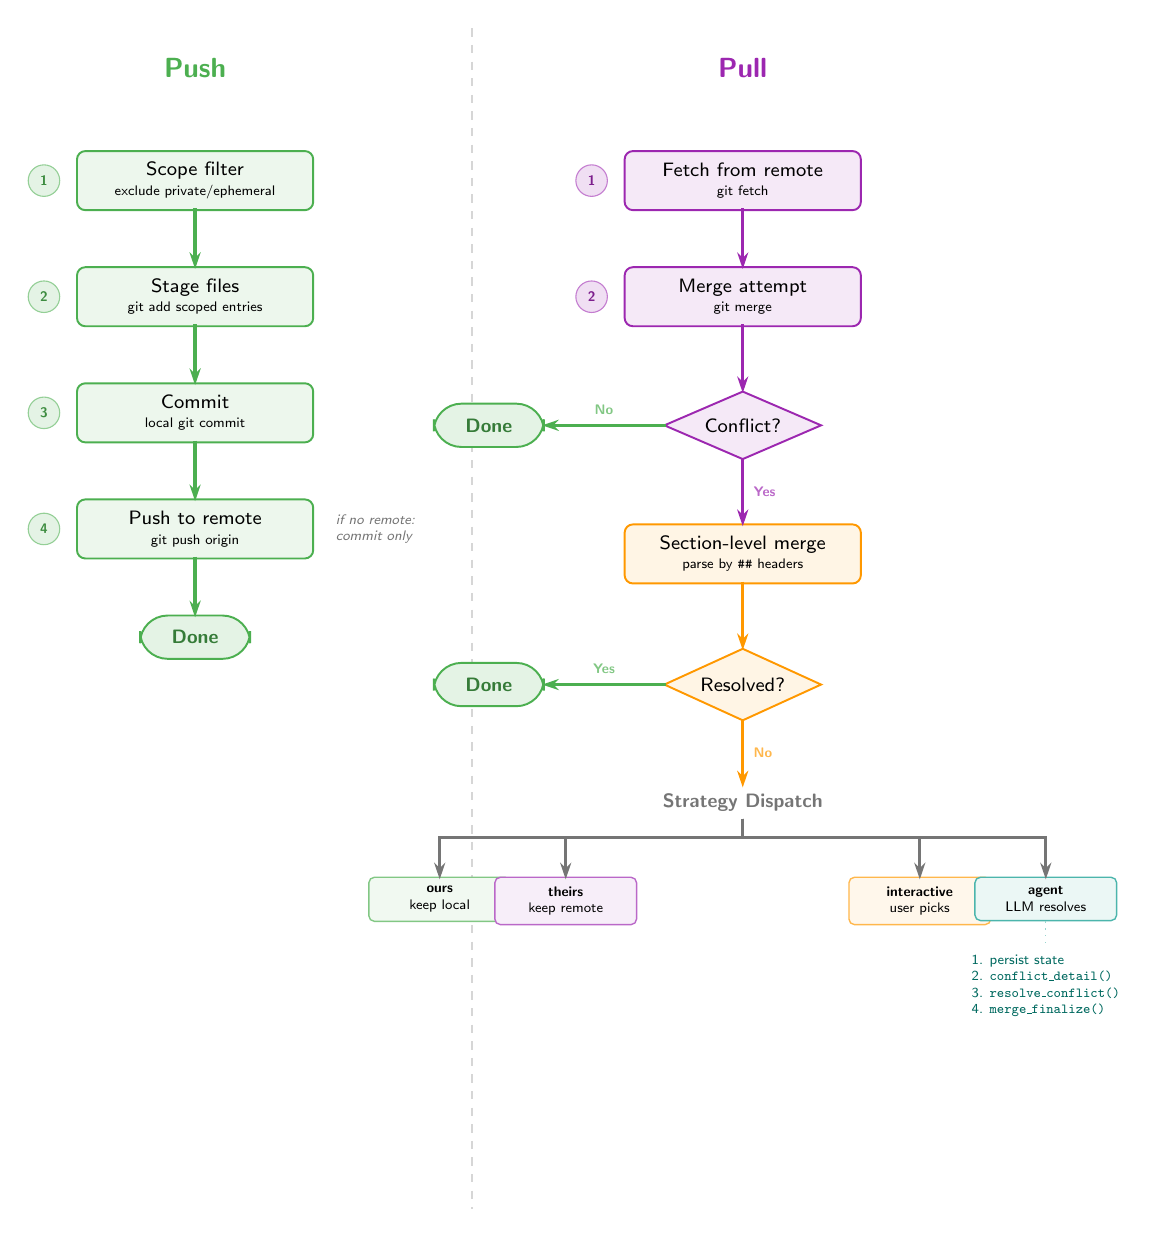
\begin{tikzpicture}[
    >=Stealth,
    every node/.style={font=\sffamily\small},
    step/.style={
        draw=#1, fill=#1!10, rounded corners=3pt,
        minimum width=3cm, minimum height=0.75cm,
        line width=0.7pt, align=center, font=\sffamily\scriptsize
    },
    decision/.style={
        draw=#1, fill=#1!10, diamond, aspect=2,
        minimum width=2cm, inner sep=2pt,
        line width=0.7pt, font=\sffamily\scriptsize, align=center
    },
    strategy/.style={
        draw=#1!70, fill=#1!8, rounded corners=2pt,
        minimum width=1.8cm, minimum height=0.55cm,
        line width=0.5pt, font=\sffamily\tiny, align=center
    },
    done/.style={
        draw=ifgreen, fill=ifgreen!15, rounded corners=10pt,
        minimum width=1.4cm, minimum height=0.55cm,
        line width=0.7pt, font=\sffamily\scriptsize\bfseries, text=ifgreen!70!black
    },
    colhead/.style={
        font=\sffamily\normalsize\bfseries, text=#1
    },
    arr/.style={-{Stealth[length=6pt, width=4pt]}, line width=1.2pt, color=#1,
        shorten >=-1pt, shorten <=-1pt},
    numlabel/.style={
        circle, draw=#1!60, fill=#1!15, inner sep=1pt,
        font=\sffamily\tiny\bfseries, text=#1!80!black, minimum size=0.4cm
    },
]

% === Column Headers ===
\node[colhead=ifgreen] (pushhead) {Push};
\node[colhead=syncpurple, right=6cm of pushhead] (pullhead) {Pull};

% Separating line
\draw[dashed, color=fsgray!30, line width=0.5pt]
    ($(pushhead.east)!0.5!(pullhead.west)+(0,0.5)$) --
    ($(pushhead.east)!0.5!(pullhead.west)+(0,-14.5)$);

% ============================
% PUSH COLUMN (left)
% ============================
\node[step=ifgreen, below=0.8cm of pushhead] (p1) {Scope f{}ilter\\[-1pt]\tiny exclude private/ephemeral};
\node[numlabel=ifgreen, left=0.2cm of p1.west] {1};

\node[step=ifgreen, below=0.7cm of p1] (p2) {Stage f{}iles\\[-1pt]\tiny git add scoped entries};
\node[numlabel=ifgreen, left=0.2cm of p2.west] {2};

\node[step=ifgreen, below=0.7cm of p2] (p3) {Commit\\[-1pt]\tiny local git commit};
\node[numlabel=ifgreen, left=0.2cm of p3.west] {3};

\node[step=ifgreen, below=0.7cm of p3] (p4) {Push to remote\\[-1pt]\tiny git push origin};
\node[numlabel=ifgreen, left=0.2cm of p4.west] {4};

\node[done, below=0.7cm of p4] (pdone) {Done};

\draw[arr=ifgreen] (p1) -- (p2);
\draw[arr=ifgreen] (p2) -- (p3);
\draw[arr=ifgreen] (p3) -- (p4);
\draw[arr=ifgreen] (p4) -- (pdone);

% No remote annotation
\node[font=\sffamily\tiny\itshape, text=fsgray, right=0.15cm of p4.east, anchor=west, align=left]
    {if no remote:\\commit only};

% ============================
% PULL COLUMN (right)
% ============================
\node[step=syncpurple, below=0.8cm of pullhead] (q1) {Fetch from remote\\[-1pt]\tiny git fetch};
\node[numlabel=syncpurple, left=0.2cm of q1.west] {1};

\node[step=syncpurple, below=0.7cm of q1] (q2) {Merge attempt\\[-1pt]\tiny git merge};
\node[numlabel=syncpurple, left=0.2cm of q2.west] {2};

\draw[arr=syncpurple] (q1) -- (q2);

% Conflict decision
\node[decision=syncpurple, below=0.8cm of q2] (qconf) {Conf{}lict?};
\draw[arr=syncpurple] (q2) -- (qconf);

% No conflict -> done
\node[done, left=1.5cm of qconf] (qdone1) {Done};
\draw[arr=ifgreen] (qconf.west) -- node[above, font=\sffamily\tiny\bfseries, text=ifgreen!70] {No} (qdone1);

% Yes -> section merge
\node[step=adaptorange, below=0.8cm of qconf] (qsec) {Section-level merge\\[-1pt]\tiny parse by \texttt{\#\#} headers};
\draw[arr=syncpurple] (qconf.south) -- node[right, font=\sffamily\tiny\bfseries, text=syncpurple!70] {Yes} (qsec);

% Resolved?
\node[decision=adaptorange, below=0.8cm of qsec] (qres) {Resolved?};
\draw[arr=adaptorange] (qsec) -- (qres);

% Yes -> done
\node[done, left=1.5cm of qres] (qdone2) {Done};
\draw[arr=ifgreen] (qres.west) -- node[above, font=\sffamily\tiny\bfseries, text=ifgreen!70] {Yes} (qdone2);

% No -> strategy dispatch
\node[font=\sffamily\scriptsize\bfseries, text=fsgray, below=0.8cm of qres] (strat) {Strategy Dispatch};
\draw[arr=adaptorange] (qres.south) -- node[right, font=\sffamily\tiny\bfseries, text=adaptorange!70] {No} (strat);

% Four strategies
\node[strategy=ifgreen, below left=0.7cm and 1.8cm of strat] (sours) {\textbf{ours}\\keep local};
\node[strategy=syncpurple, below left=0.7cm and 0.2cm of strat] (stheirs) {\textbf{theirs}\\keep remote};
\node[strategy=adaptorange, below right=0.7cm and 0.2cm of strat] (sinter) {\textbf{interactive}\\user picks};
\node[strategy=domteal, below right=0.7cm and 1.8cm of strat] (sagent) {\textbf{agent}\\LLM resolves};

\draw[arr=fsgray] (strat.south) -- ++(-0.0,-0.2) -| (sours.north);
\draw[arr=fsgray] (strat.south) -- ++(-0.0,-0.2) -| (stheirs.north);
\draw[arr=fsgray] (strat.south) -- ++(-0.0,-0.2) -| (sinter.north);
\draw[arr=fsgray] (strat.south) -- ++(-0.0,-0.2) -| (sagent.north);

% Agent sub-flow
\node[font=\sffamily\tiny, text=domteal!70!black, align=left, below=0.3cm of sagent.south, anchor=north]
    (agentflow) {
        1. persist state\\
        2. \texttt{conf{}lict\_detail()}\\
        3. \texttt{resolve\_conf{}lict()}\\
        4. \texttt{merge\_f{}inalize()}
    };
\draw[dotted, color=domteal!40, line width=0.5pt] (sagent.south) -- (agentflow.north);

\end{tikzpicture}
\end{document}
